\chapter{Top Up Procedure and Analysis} \label{app_topup_procedure_analy}

\section{Overview of the Top Up Code}
As described in chapter \ref{chap_topup}, the top up calculation is done by firstly establishing correct level correpondance between BPRM and RDW calculation, and this ensures extending the correct tail, adding the contribution from the correct other target configurations, and including the correct unincluded bound levels. In the flowchart \ref{fig_topup_flowchart}, as you can see, the main procedure is divided into two parts, one focues on the matching step, and the other on the top up step. In the matching step, which starts in directory \textbf{\textit{match/}}, we need to firstly finish the RDW calculation with only the core configurations included in BPRM calculation, and the scripts in direcotries \textbf{\textit{bound\_levels\_0/}}, \textbf{\textit{create\_mesh\_1/}} and \textbf{\textit{generate\_PI\_2/}} will extract the bound levels, create energy mesh for each level and generate the photoionization cross section, respectively. Now we are ready to do the matching. Since BPRM code categorizes the bound levels by $2J$ and $\pi$, and these levels are sorted in energy-ascending order, the script in \textbf{\textit{bound\_levels\_0/}} just does this job, and the photoionization cross section are generated in the same order. Thus we can just blindly match the levels in BPRM and RDW calculations by level index and plot the photoionization cross section against each other. Usually we get a roughly good match, and the RDW cross section does reproduce the background of BPRM calculation very well. However, as illustrated in section \ref{section_matching}, due to the energies being closely packed in a small region, these levels can not be distinguished by energy, and we should carefully inspect the matching of the photoionization cross section. Once we decide to match level $m$ in BPRM calculation with level $n$ in RDW calculation, and level $n$ in BPRM with level $m$ in RDW, we put such pairs $m~~n$ and $n~~m$ in each line in file \textbf{\textit{correct\_match\_n4}}, and replot the photoionization cross section. Such iteration is repeated until satisfatory result is achieved. In section \ref{section_matching}, I mentioned a ``fake'' level found in BPRM calculation, and I assigned one level in RDW twice to the two almost the same levels in BPRM. When all levels are matched, the correction to the matching should be stored in folder $correct\_match\_n3$ or $correct\_match\_n4$ with names as $2J\_\pi$. The complete result can be found at \url{https://github.com/zhao1157/PhD-Atomic-Physics/tree/master/fe17_fe18_matched_levels} for both \ion{Fe}{xvii} and \ion{Fe}{xviii}. And these level information, especially the configuration, can be readily extracted. In $ratio\_analysis\_4$, we can utilized the matched levels and categorize them in terms of ratio of BPRM/RDW at the last point. For more details, see section \ref{section_detailed_topup_code}. I also put the bound-bound top up calculation inside $match/$ because of the identified levels in $level\_identification\_3/$. 

Once levels are appropriately matched, we are all set to proceed the top up calculation, i.e. extending the tail, adding the contribution from other core configurations, and including the levels that are missed out. In folder $topup/$, the level matching correction information from $match/$ is needed here. To extend the tail,we need to find the last energy point in each level in BPRM calculation, which decides the starting point at which we need to create new energy mesh, and its lowest ionizaiton threshold, i.e. the absolute value of its energy, which decides the end of the energy mesh, i.e. $500~Ry$ more than the lowest ionization threshold. And this is done in $extract\_bprm\_tail\_n4\_0/$. Then we need to do RDW calculation including the other core configurations only, and extract these new thresholds for each level and sort them in ascending order and find the ones that are beyond the last point in BPRM calculation. The tail energy mesh is created with these new thresholds and 10 points are assigned between adjacent thresholds, and a few hundred of points between the last threshold and the maximum energy point, i.e.  $500~Ry$ more than the lowest ionization threshold which is found in $extract\_bprm\_tail\_n4\_0/$. In \textbf{\textit{generate\_PI\_2/}}, the RRTable should be the one containing only the core configurations included in BPRM. In \textbf{\textit{combine\_tail\_3/}}, these tails are added to BPRM data. Now we are ready to add the contribution from other core configurations to the tailed BPRM data. Obviously we need to use the RRTable including only the other core configurations, and be aware that there are cases where there are no transitions from some levels to these core configurations, so we add nothing. For those levels which do have extra transitions due to these core configurations, we find the lowest threshold for each level and extract the energy mesh from the tailed BPRM data that is larger than the lowest threshold. After the calculation is done, the whole data can be combined in \textbf{\textit{combine\_other\_targets\_3/}}. By far the complete data has been obtained for those levels included in BPRM calculation. 

As stated in chapter \ref{chap_topup}, the bound levels are counted with principle quantum number wihthin 10, so we exclude the levels that have been included in BPRM calculation, and collect the rest. This is done in \textbf{\textit{other\_levels\_2/}}. The complete photoionization cross section is plotted and accessible at \url{https://github.com/zhao1157/PhD-Atomic-Physics/tree/master/fe17_fe18_full_data}. In addition, I also wrote a script that can extract the transition information for one level in \textbf{\textit{extract\_free\_config\_3/}}. To find the transition information for the jumps of all levels, go to \textbf{\textit{extract\_jump\_4/}}.

%===== FLOWCHART
\begin{figure}
	\centering
	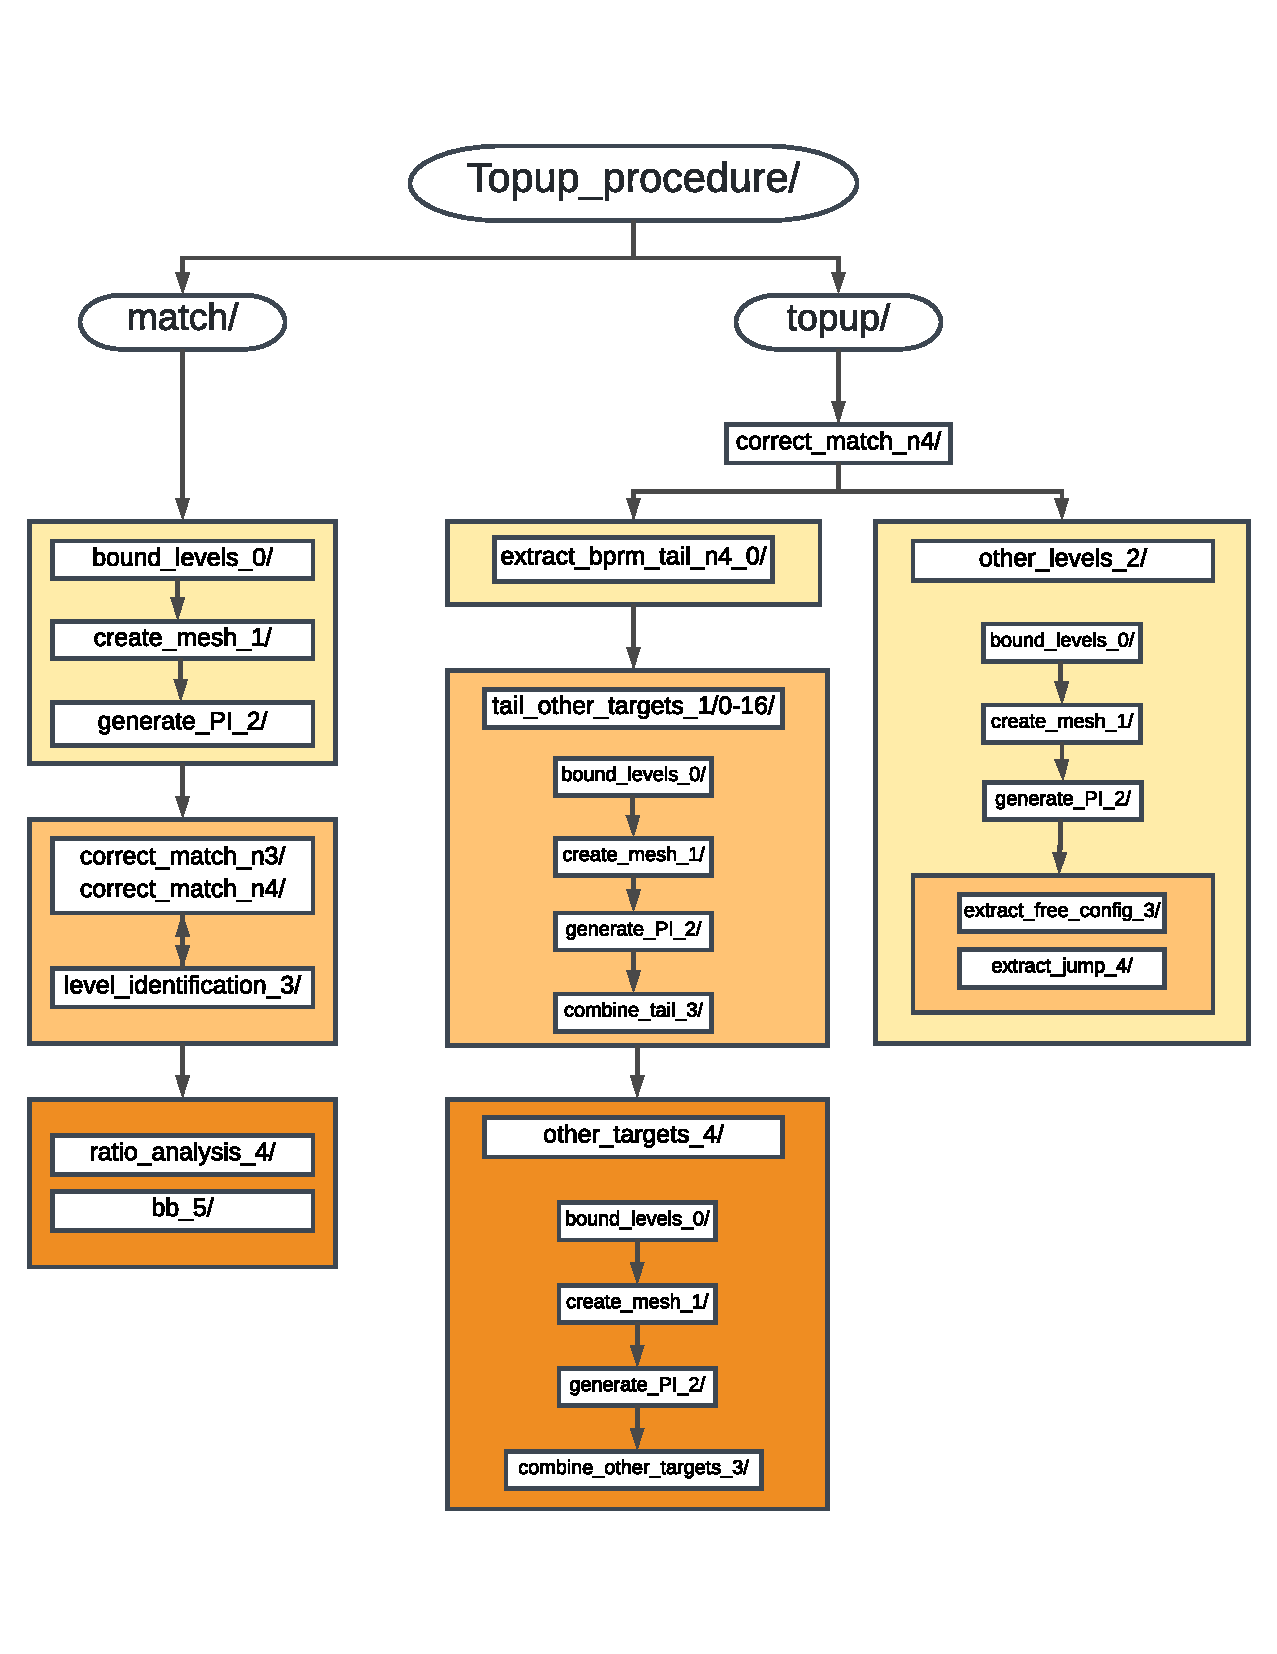
\includegraphics[width=1.0\textwidth]{app_1/figures/topup_procedure_flowchart}
	\caption{The architecture of the code that is written for the top up calculation and analysis. It is available in \url{https://github.com/zhao1157/PhD-Atomic-Physics}.}
	\label{fig_topup_flowchart}
\end{figure}

\section{Detailed Description of the Top Up Code}
\label{section_detailed_topup_code}
Since this top up procedure is divided into several parts and in each part there are a few separate scripts needed to be executed, the names of these parts and scripts implicitly tells the relative order of executing them. For example, folders \textbf{\textit{bound\_levels\_0/}}, \textbf{\textit{create\_mesh\_1/}} and \textbf{\textit{generate\_PI\_2/}} have to executed in the order as the last index before `\_' indicates. And the scripts in \textbf{\textit{create\_mesh\_1/}}, i.e. \textbf{\textit{extract\_trans\_awk\_1.sh}}, \textbf{\textit{collect\_thresh\_awk\_2.sh}}, \textbf{\textit{order\_thresh\_awk\_3.sh}}, \textbf{\textit{add\_mini\_diff\_awk\_4.sh}} and  \textbf{\textit{creat\_fine\_mesh\_5.py}}, have to be executed in the order as the index between `\_' and the extension of the file name indicates. The following is a detailed description of the important scripts.

\subsection{\textit{match/}}
\begin{enumerate}
	\item \textbf{\textit{bound\_levels\_0/}}: extract the bound levels that contribute to the photoionization cross section, in terms of $2J$ and $\pi$.
		\begin{itemize}
			\item \textit{extract\_bound\_levels\_0.py}: input the files that contain the energy and RRTable, the number of electrons of the bound configurations, the charge of the core confgurations, and the energy of the ground state of the core configurations in unit of ev. Note it is more accurate to use the energy of the ground state of the core with same-n-complex configuration interaction, though different-n-complex configuration interaction of the core configurations is used to maximally reproduce the background of BPRM calculation. It outputs the levels in energy ascending order for each symmetry $2J\_\pi$, and the negative and positive levels are separated.
		\end{itemize}
		
	\item \textbf{\textit{create\_mesh\_1/}}: create energy mesh for each bound state level. To delineate the edges, 10 points are uniformly assigned between adjacent thresholds.
		\begin{itemize}
			\item \textit{extract\_trans\_awk\_1.sh}: collect the transition information for the levels of interest, i.e. the header line for each transition. Usually we need to create a symlink that points to a file which contains the levels we are interested in, e.g. \colorbox{gray!20} {\textit{ln -s ../bound\_levels\_0/0\_0\_neg bound\_levels\_0}} (see script \textit{run\_JJ\_Pi.sh} in \textbf{\textit{match/}} below).
			\item \textit{collect\_thresh\_awk\_2.sh}:  collect the various thresholds for each level, and output the level index and its thresholds in one single line.
			\item \textit{order\_thresh\_awk\_3.sh}: sort the thresholds for each level in ascending order, and append each level with an energy that is 105 Ry (or another range of your interest) more than the lowest threshold, and remove other thresholds that are the same as one threshold.
			\item \textit{add\_mini\_diff\_awk\_4.sh}: append the smallest difference between adjacent thresholds at the end of each line for each level. This value is useful when creating energy mesh and 10th of it is used as the increment. So in this way we try to delineat the edges of various transitions.
			\item \textit{creat\_fine\_mesh\_5.py}: create an energy mesh for each level, with 10 points in any adjacent shresholds, and 20 points between the last threshold and the maximal energy point.
			\item \textit{test\_same.awk}:  it is called inside of \textit{creat\_fine\_mesh\_5.py} to test the fine mesh whether the adjacent points are the same or not. Usually I do not use it.
			\item \textit{run.sh}: show the order of executing the scripts above. It is usually called in a loop to run these steps.
		\end{itemize}
	
	\item \textbf{\textit{generate\_PI\_2/}}: after mesh being generated, the scripts in this folder calculate the photoionization cross section.
		\begin{itemize}
			\item \textit{fe18\_n3.py}:  load the existing energy binary file and RRTable binary file and interpret and extrapolate the photoionization cross section for each level in the energy mesh created in \textit{create\_mesh\_1/}. In this script, we use \textit{fac.InterpCross()} to output the data for each transition and then to do the summation over all transitions for each level. We can also use \textit{fac.TotalPICross()} to get the summed result, but in many situtations the energy mesh and number of transitions are large which results in the large memory requirement. Thus we abandon it in general.
			\item \textit{add\_awk.sh}: after \textit{fac.InterpCross()} generates the data for all transitions, it reads the data and sums it up in unit of $Mb$.
		\end{itemize}
	
	\item \textit{run\_JJ\_Pi.sh}: after the bound levels are extracted in directory \textbf{\textit{bound\_levels\_0/}}, we are ready to generate the photoionization cross section for each level in each symmetry category $2J\_\pi$.
	
	\item \textbf{\textit{level\_identification\_3/}}: As the levels are sorted in energy-ascending order for each symmetry $2J\_\pi$ just as in BPRM calculation, we are ready to just plot the the photoionization cross section of RDW and BPRM. While checking how well they match, we need to make sure the energy agrees well. In some situations, we need to switch or shift the levels so that they are matched. After finishing matching the levels, we are ready to print out the level information and find out the configuraiton of each level.
		\begin{itemize}
			\item \textit{plot\_n4\_background\_1.py}: plot the photoionization cross section of RDW and BPRM and see how well they match with each other. Correction is needed if they don't agree well by switching or shifting to other reasonable levels. File \textit{correct\_match\_n4} or \textit{correct\_match\_n3}, where n3 or n4 refers to n=3 or n=4 core configuraitons, contains the information of level switching. These numbers represent the LINE NUMBER of the level in \textit{../bound\_levels\_0/2J\_$\pi$\_neg} file, assuming the BPRM levels are also written in a file in the same format. In the script, we need to set the number of levels in the symmetry of interest in BPRM calculation. Usually the number of levels obtained in BPRM calculation is no more than that got from RDW. Required is the number of lines that contain the energies of the core states in the front of each level data set in BPRM calculation.
			\item \textit{level\_identification\_2.py}: in this script, the file that contains the correction in matching step is needed, and variable $level\_JJ\_Pi$ is a dictionary contains $2J\_\pi~:~number\_of\_levels\_in\_BPRM$.
			\item \textit{cat.sh}: a simple script to concatenate the level information into a single file that is needed in 
		\end{itemize}
	
	\item \textbf{\textit{ratio\_analysis\_4/}}: extract the information of the levels whose ratios fall within a range. This script is useful if you want to get a rough idea of how well the calculation of BPRM and RDW agrees with each other at the last point, and what kind of levels do well and not well. The order of the levels written in files \textit{level\_file} and \textit{ratio\_file} has to be the same. Usually it is $0\_0$ ($2J\_\pi$), $0\_1$, $2\_0$, $2\_1$, ..., $16\_0$, $16\_1$ for \ion{Fe}{xvii}, but of course it can vary as long as they are in the same fashion in these two files.
	\begin{itemize}
		\item \textit{ratio\_configurations.py}: it collects the levels whose ratio $<0.5$ in 0, $>=0.5~\&<1.5$ in 1, $>=1.5~\&<2.5$ in 2, etc., the rest of levels in n (in line 8, \colorbox{gray!20}{\textit{ratios = range(n)}}).
	\end{itemize}
	
	\item \textbf{\textit{bb\_5/}}: does the bound-bound top up calculation.
	\begin{itemize}
		\item \textit{create\_e\_file.py}: create e-file needed in opacity calculation. In line 7, variable $ind\_max\_remove$ represents the maximum level index that bound-quasi-bound transitions should be neglected as they are already included in BPRM. In the $fac.Structure()$ part, the bound configurations have to be in front of the other quasi-bound configurations. In line 73, it excludes the transitions that are from the positive-energy levels, the transitions that have already been included in BPRM stgbb, and the ones that have already been included in bound-free, i.e. resonances due to $n=2$ core configurations coupled with an outer electron. In list $file\_en\_454\_rest$, the first file has to be energy file, followed by the transition files. These transition files have to share the same energy file, otherwise when reading different transition files, levels will be messed up.
		\item \textit{create\_f\_file.py}: creates f-file needed in opacity calculation. The same variable settings as in file \textit{create\_e\_file.py}.
	\end{itemize}
\end{enumerate}

\subsection{\textit{topup/}}
\begin{enumerate}
	\item \textbf{\textit{extract\_bprm\_tail\_n4\_0/}}
		\begin{itemize}
			\item \textit{extract\_bprm\_0.py}: used to extract the threshold and last point for each level in bprm data for tail-processing. The threshold is used to determine the highest energy point, i.e. $500~Ry$ more than the threshold. The last point is used to compare with various thresholds in order to determine the thresholds that are beyond this point.
		\end{itemize}
	
	\item \textbf{\textit{tail\_other\_targets\_1/0-16/}}
		\begin{enumerate}
			\item \textbf{\textit{bound\_levels\_0/}}: only consider the transitions to other core configurations as we want to extract the thresholds due to them, so that the energy mesh can be created appropriately.
				\begin{itemize}
					\item \textit{extract\_bound\_levels\_0.py}: the same as the one in \textbf{\textit{match/bound\_levels\_0/}}.
				\end{itemize}
		
			\item \textbf{\textit{create\_mesh\_1/}}: the filenames of these scripts are the same as those in 
			\textbf{\textit{match/create\_mesh\_1/}}, but the content can be drastically different.
				\begin{itemize}
					\item \textit{extract\_trans\_awk\_1.sh}: the same as those in \textbf{\textit{match/create\_mesh\_1/}}.
					\item \textit{collect\_thresh\_awk\_2.sh}: the same as those in \textbf{\textit{match/create\_mesh\_1/}}.					
					\item \textit{order\_thresh\_awk\_3.sh}: compared with the one in \textbf{\textit{match/create\_mesh\_1/}}, line 19 is commented out in the current version, because the lowest threshold for each level is stored in \textbf{\textit{extract\_bprm\_tail\_n4\_0/}}.					
					\item \textit{add\_mini\_diff\_awk\_4.sh}: the same as those in \textbf{\textit{match/create\_mesh\_1/}}.			
					\item \textit{creat\_fine\_mesh\_5.py}: due to the correction in matching step, we first reorder the levels obtained from \textit{add\_mini\_diff\_awk\_4.sh}, and then determine how to create the energy mesh. If all the thresholds are within the last point of BPRM calculation, then we simply assign 400 points between the last point and the point which is 500 Ry above the threshold obtained in \textbf{\textit{extract\_bprm\_tail\_n4\_0/}}. Otherwise, we find the threshold that just starts to become larger than the last point, and assign 10 points between the last point and that threshold, and also 10 points between the following thresholds, and 300 points between the last threshold and the point which is $500~Ry$ above the threshold obtained in \textbf{\textit{extract\_bprm\_tail\_n4\_0/}}.					
					\item \textit{test\_same.awk}: the same as those in \textbf{\textit{match/create\_mesh\_1/}}.					
					\item \textit{run.sh}: it is slightly different from the one in \textbf{\textit{match/create\_mesh\_1/}}, in that \textit{creat\_fine\_mesh\_5.py} needs to read some input parameters, i.e. $2J$ and $\pi$.					
				\end{itemize}
			
			\item \textbf{\textit{generate\_PI\_2/}}: since we are extending the tail, which is due to the core configuraitons that are included BPRM calculation, only these core configuraitons are considered.
				\begin{itemize}
						\item \textit{fe18\_n3.py}: the same as those in \textbf{\textit{match/generate\_PI\_2/}}.		
						\item \textit{add\_awk.sh}: the same as those in \textbf{\textit{match/generate\_PI\_2/}}.
				\end{itemize}
			\item \textbf{\textit{combine\_tail\_3/}}: attach the RDW tail to BPRM.
				\begin{itemize}
					\item \textit{combine\_tail.py}: since the levels have already been corrected, we are ready to just concatenate the tail to BPRM data. Note, in this script, we can get the ratio of BPRM/RDW at the last point, which can give us a rough idea of how these two calculation compare with each other. Through this ratio, we can find the levels that are doing well and not well using script in \textbf{\textit{match/ratio\_analysis\_4/}}. To activate this option, uncomment out line 34, and comment out line 35.
					\item \textit{cat.sh}: simply to concatenate $2J\_\pi\_ratio$ files into one file ratio, which is needed in \textbf{\textit{match/ratio\_analysis\_4/}}.
				\end{itemize}
			\item \textbf{\textit{other\_targets\_4/}}: We are going to add the contribution from other core configurations to the tailed-BPRM data. Before proceeding, we need to create a symlink in this directory to \textbf{\textit{../bound\_levels\_0/}}, i.e. \colorbox{gray!20}{\textit{ln -s ../bound\_levels\_0/}}, because the bound level information is the same.
				\begin{enumerate}
					\item \textbf{\textit{create\_mesh\_1/}}: extract the energy mesh for each level.
						\begin{itemize}
							\item \textit{extract\_trans\_awk\_1.sh}: the same as those in \textbf{\textit{match/create\_mesh\_1/}}.
							\item \textit{collect\_thresh\_awk\_2.sh}: the same as those in \textbf{\textit{match/create\_mesh\_1/}}.		
							\item \textit{order\_thresh\_awk\_3.sh}: comment out line 19, as the mesh has already been created, now we just need to find the lowest threshold, and extract the energy mesh.
							\item \textit{extract\_mesh\_4.py}: we take note of the energy index at which the contribution from other core configurations starts to kick in in each level and the rest of the energy points are the mesh we need. And there are cases where there are no transitions to these core configurations, so we denote it as \textit{skip}. These information will be needed when adding the extra contribution to the tailed-BPRM data.
							\item \textit{run.sh}: run the first three scripts.
						\end{itemize}
					\item \textbf{\textit{generate\_PI\_2/}}: calculate the photoionization cross section.
						\begin{itemize}
							\item \textit{fe18\_n3.py}: the same as those in \textbf{\textit{match/generate\_PI\_2/}}.		
							\item \textit{add\_awk.sh}: the same as those in \textbf{\textit{match/generate\_PI\_2/}}.
						\end{itemize}
					\item \textbf{\textit{combine\_other\_targets\_3/}}
						\begin{itemize}
						\item \textit{combine\_other\_targets.py}: combine the tailed-BPRM data with those in \textbf{\textit{generate\_PI\_2/}}.	
						\item \textit{cat.sh}: simply concatenate the these data into one file.
					\end{itemize}
				\end{enumerate}
		\end{enumerate}
	\item \textbf{\textit{other\_levels\_2/}}: We are going to collect all the other bound levels and calculate the photoionization cross section due to all the core configurations included in BPRM calculation and the above top up calculation.
		\begin{enumerate}
			\item \textbf{\textit{bound\_levels\_0/}}: 
				\begin{itemize}
					\item \textit{extract\_bound\_levels\_0.py}: the same as those in \textbf{\textit{match/bound\_levels\_0/}}.		
					\item \textit{extract\_other\_levels\_1.py}:extract all the other bound levels that are not included in BPRM calculation. Note the correction in matching is needed, and variable \textit{sym\_level} is a dictionary containing $2J\_\pi~:~number\_of\_levels\_in\_BPRM$.
					\item \textit{create\_e\_file.py}: create the e-file needed in opacity calculation for these bound levels. Variable $ind\_base$ is the number of bound levels included in BPRM calculation, so the unincluded bound levels are indexed based on that number.
				\end{itemize}
			\item \textbf{\textit{create\_mesh\_1/}}: 
				\begin{itemize}
					\item \textit{extract\_trans\_awk\_1.sh}: the same as those in \textbf{\textit{match/create\_mesh\_1/}}.
					\item \textit{collect\_thresh\_awk\_2.sh}: the same as those in \textbf{\textit{match/create\_mesh\_1/}}.
					\item \textit{order\_thresh\_awk\_3.sh}: the same as those in \textbf{\textit{match/create\_mesh\_1/}}.
					\item \textit{add\_mini\_diff\_awk\_4.sh}: the same as those in \textbf{\textit{match/create\_mesh\_1/}}.	
					\item \textit{creat\_fine\_mesh\_5.py}: compared with the one in \textbf{\textit{match/create\_mesh\_1/}}, it differs in the way of assigning the points between adjacent thresholds. If the difference is within $10~ev$, then 10 points, othewise 20.
					\item \textit{split.sh}: split the energy mesh into a few files, each of which contains 1000 levels. This might be helpful when there are so many levels and the number of transitions is huge, so we can split the calculation in a few chunks and run them simultaneously. 1000 can be changed to other values.
					\item \textit{test\_same.awk}: the same as those in \textbf{\textit{match/create\_mesh\_1/}}.
					\item \textit{run.sh}: run the above scripts.	
				\end{itemize}
			\item \textbf{\textit{generate\_PI\_2/}}:
				\begin{itemize}
					\item \textit{fe18\_n4.py}: it is essentially the same as the one in \textbf{\textit{match/generate\_PI\_2/}}, but it differs a bit in that it reads an input and the file path changes a bit.
					\item \textit{add\_awk.sh}: the same as the one in \textbf{\textit{match/generate\_PI\_2/}}.
					\item \textit{create\_run\_0.sh}: creates PBS jobs for computation of differents chunks. 1000 should be changed if it is changed in \textit{create\_mesh\_1/split.sh}.
					\item \textit{check\_zero\_1.py}: remove the entries that has photoionization cross section of 0.
					\item \textit{combine\_head\_data\_2.py}: it needs a file called head that contains the same energy of the core configurations as in BPRM calculation, and a file containing the level information, i.e. \colorbox{gray!20} {ln -s ../bound\_levels\_0/neg levels}.
				\end{itemize}
			\item \textbf{\textit{extract\_free\_config\_3/}}:
				\begin{itemize}
					\item \textit{extract\_free\_config.py}:  it finds the transitions that contribute most of the photoionization cross section for a level in a given range ($en\_start$, $en\_end$). $exp\_pi$ is a list that contains the exponents of the photoionization cross section.
				\end{itemize}
			\item \textbf{\textit{extract\_jump\_4/}}: to analysis the PEC\_L\_Edge transitions.
				\begin{itemize}
					\item \textit{extract\_jump\_start\_end\_1.py}: extract the PEC\_L\_Edge main transitions for each level. The output file is named as $level\_exp$, e.g. $100\_+01$, in which written are the transitions from level 100 with a magnitude of $10^{+01}$ at the first default energy point.
					\item \textit{extract\_jump\_start\_end\_2.py}: print out the level index, the first and last thresholds for all levels, which are grouped as the principle quantum number of the outer electron.
					\item \textit{extract\_jump\_start\_end\_3.py}: extract the photoionization cross section near the ``last'' threhold and $500~Ry$.
				\end{itemize}
			
		\end{enumerate}
\end{enumerate}

